\documentclass{article}

\usepackage{graphicx}
\usepackage{tikz}
\usepackage{tikzsymbols}
\usetikzlibrary{calc,patterns,shapes.geometric}
\pagestyle{empty}
\usepackage[margin=0pt]{geometry}
\geometry{papersize={14in,12in}}

\def\centerarc[#1](#2)(#3:#4:#5){\draw[#1] ($(#2)+({#5*cos(#3)},{#5*sin(#3)})$) arc (#3:#4:#5);}

\begin{document}
	\begin{figure}
		\centering
		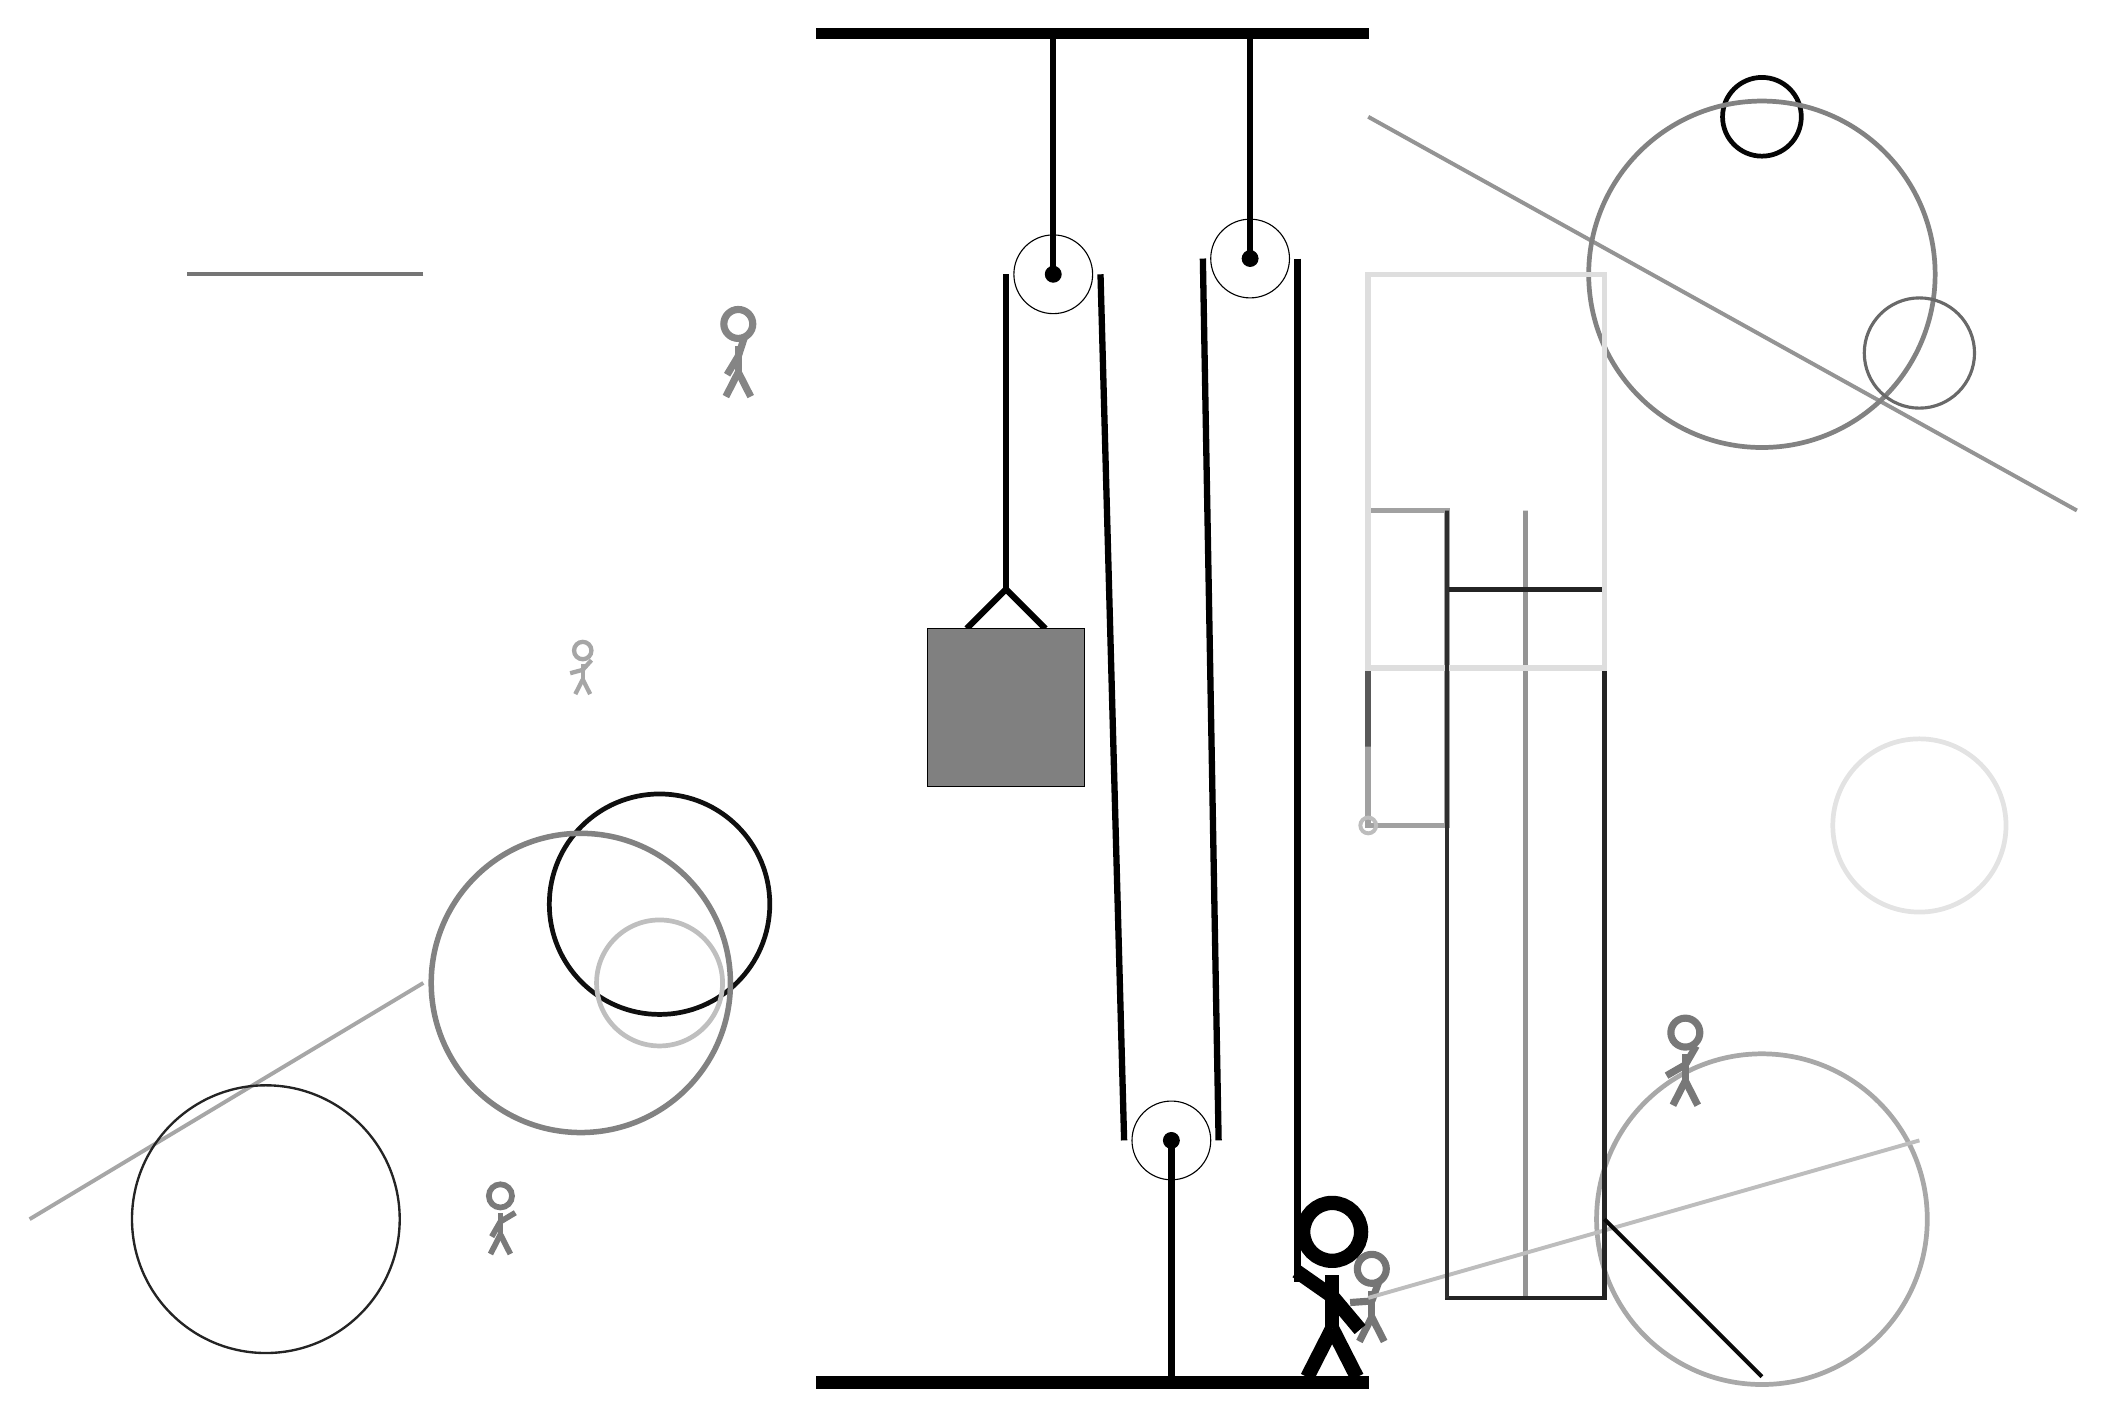
\begin{tikzpicture}
			%%%%% START %%%%%
			
			\draw[fill=black] (-2, 14) rectangle (5, 14.125);
			
			\draw (1, 11) circle (0.5);
			\draw[fill=black] (1, 11) circle (0.1);
			\draw[line width=0.8mm]  (1, 14) -- (1, 11);
			
			\draw[line width=0.7mm, color=black!37] (6, 8) rectangle (5, 4);
			
			\draw [line width=0.5mm, color=black!26](5, 4) circle (0.1);
			\draw [line width=0.6mm, color=black!34](10, -1) circle (2.1);
			\draw [line width=0.6mm, color=black!94](-4, 3) circle (1.4);
			
			\node[line width=0.6mm, color=black!54] at (5, -2) {\Strichmaxerl[5][4][70]};
			
			\node[line width=0.3mm, color=black!35] at (-5, 6) {\Strichmaxerl[3][15][48]};
			\draw [line width=0.7mm, color=black!49](-5, 2) circle (1.9);
			\draw[line width=0.6mm, color=black!42] (7, -2) rectangle (7, 8);
			\node[line width=0.4mm, color=black!53] at (9, 1) {\Strichmaxerl[5][30][60]};
			
			\draw[line width=0.5mm, color=black!42](5, 13) -- (14, 8);
			
			\draw [line width=0.6mm, color=black!11](12, 4) circle (1.1);
			\draw [line width=0.6mm, color=black!25](-4, 2) circle (0.8);
			\draw [line width=0.6mm, color=black!98](10, 13) circle (0.5);
			
			\draw[line width=0.5mm, color=black!35](-7, 2) -- (-12, -1);
			\draw[line width=0.5mm, color=black!26](5, -2) -- (12, 0);
			\draw[line width=0.6mm, color=black!86] (6, -2) rectangle (8, 7);
			
			\draw [line width=0.6mm, color=black!49](10, 11) circle (2.2);
			\draw[line width=0.5mm, color=black!54](-7, 11) -- (-10, 11);
			\draw[line width=0.5mm, color=black!96](10, -3) -- (8, -1);
			\draw[line width=0.7mm, color=black!65] (5, 10) rectangle (5, 5);
			\draw [line width=0.3mm, color=black!86](-9, -1) circle (1.7);
			
			\draw[line width=0.7mm, color=black!13] (5, 11) rectangle (8, 6);
			\node[line width=0.5mm, color=black!48] at (-3, 10) {\Strichmaxerl[5][59][72]};
			\draw [line width=0.4mm, color=black!59](12, 10) circle (0.7);
			\node[line width=0.5mm, color=black!52] at (-6, -1) {\Strichmaxerl[4][60][31]};
			
			\draw[line width=0.5mm, color=black!82] (6, -2) rectangle (6, 8);
			
			\draw[fill=white](2.5, 0) circle (0.5);
			\draw[fill=black] (2.5, 0) circle (0.1);
			\draw[line width=0.8mm]  (2.5, -3) -- (2.5, 0);
			
			\draw[fill=white](3.5, 11.2) circle (0.5);
			\draw[fill=black] (3.5, 11.2) circle (0.1);
			\draw[line width=0.8mm] (3.5, 14) -- (3.5, 11.2);
			
			\draw[line width=0.8mm] (-0.1, 6.5) -- (0.4, 7.0) -- (0.9, 6.5);
			\draw[fill=black!50] (-0.6, 6.5) rectangle (1.4, 4.5);
			
			\draw[line width=0.8mm] (0.4, 11) -- (0.4, 7.0);
			\centerarc[line width=0.8mm](1, 11)(0:180:0.6);
			\draw[line width=0.8mm](1.6, 11) -- (1.9, 0);
			\centerarc[line width=0.8mm](2.5, 0)(180:360:0.6);
			\draw[line width=0.8mm](3.1, 0) -- (2.9, 11.2);
			\centerarc[line width=0.8mm](3.5, 11.2)(0:180:0.6);
			\draw[line width=0.8mm](4.1, 11.2) -- (4.1, -1.8);
			
			\node at (4.5, -1.9) {\Strichmaxerl[10][-35][-50]};
			
			\draw[fill=black] (-2, -3) rectangle (5, -3.15);
			
			%%%%% END %%%%%
		\end{tikzpicture}
	\end{figure}	
\end{document}